% Name: De Morgan's law
% Description: The complements of A and B hatched in two directions: the cross-hatched region, outside both sets, shows that the complement of A ∪ B is A^c ∩ B^c.
% Tags: De Morgan's law, complement, union, intersection

\usetikzlibrary{patterns}

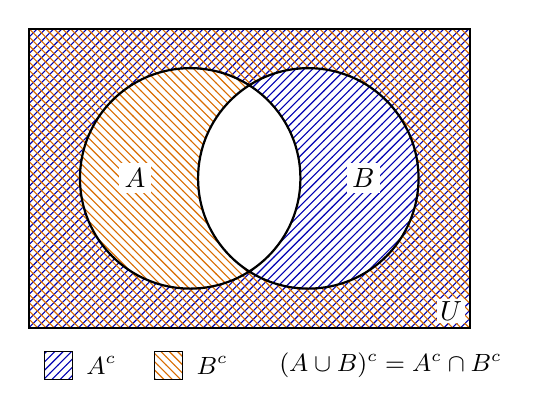
\begin{tikzpicture}[thick]
  \fill[pattern=north east lines, pattern color=blue!70!black, even odd rule] (-2.8,-1.9) rectangle (2.8,1.9) (-0.75,0) circle (1.4);
  \fill[pattern=north west lines, pattern color=orange!85!black, even odd rule] (-2.8,-1.9) rectangle (2.8,1.9) (0.75,0) circle (1.4);
  \draw (-0.75,0) circle (1.4) (0.75,0) circle (1.4);
  \draw (-2.8,-1.9) rectangle (2.8,1.9);
  \node[fill=white, inner sep=2pt] at (-1.45,0) {$A$};
  \node[fill=white, inner sep=2pt] at (1.45,0) {$B$};
  \node[fill=white, inner sep=1pt, above left] at (2.75,-1.85) {$U$};
  \draw[thin, pattern=north east lines, pattern color=blue!70!black] (-2.6,-2.55) rectangle +(0.35,0.35);
  \node[right, font=\small] at (-2.2,-2.375) {$A^c$};
  \draw[thin, pattern=north west lines, pattern color=orange!85!black] (-1.2,-2.55) rectangle +(0.35,0.35);
  \node[right, font=\small] at (-0.8,-2.375) {$B^c$};
  \node[right, font=\small] at (0.25,-2.375) {$(A \cup B)^c = A^c \cap B^c$};
\end{tikzpicture}
